%\documentclass{article}
%\documentclass[11pt]{article}   % Preset settings for two columns

\documentclass{llncs}

%\setlength{\textheight}{9.0in}
%\setlength{\textwidth}{6.5in}
%\setlength{\columnsep}{0.375in}
%\setlength{\oddsidemargin}{0.0in}
%\setlength{\topmargin}{0.0in}
%\setlength{\headheight}{0.0in}
%\setlength{\headsep}{0.0in}
%\setlength{\parindent}{1pc}

%\usepackage{doublespace}

\usepackage[pagewise]{lineno}       % For line number
\linenumbers

\usepackage{alltt}                         % For program with subscript
\usepackage[mathcal]{euscript}             % For special math symbol

\usepackage{graphicx}                      % For EPS figure
\usepackage{times}                         % For PDF font

%\usepackage{hyperref}                      % For hyper link, should be the last one 

\usepackage[ruled, vlined]{algorithm2e}    % For algorithm, 
                                           % it seems a bug make it has to be here

%\usepackage{psfig}                        % For old PS figure

%\pagestyle{empty}                         % No page Numbering
\pagestyle{plain}                         

%%%% Define theorem
%\newtheorem{theorem}{Theorem}[section]

%------------------------------------------------------------------------- 
%------------------------------------------------------------------------- 

\begin{document}

%--------------------

% title.tex

\date{}      %%%% so that date does not print.

\title{ Structure and algorithm for \\implementing OpenMP workshares}

\author{Guansong Zhang, Raul Silvera, Roch Archambault \thanks{The
    opinions expressed in this paper are those of the authors and not
    necessarily of IBM.}  }

%\thanks{The opinions expressed in this paper are those of the
%  authors and not necessarily of IBM.}


\institute{IBM Toronto Lab \\
Toronto \\
ON, L6G 1C7, Canada}

%\author{Guansong Zhang, Raul Silvera, Roch Archambault\\ 
%\\
%\small IBM Toronto Lab \\ 
%\small Toronto \\ 
%\small ON, L6G 1C7, Canada}


\maketitle

\thispagestyle{empty}

% abstract.tex

\begin{abstract}
  Barrier synchronization is an important and performance critical
  primitive in many parallel programming models, including the popular
  OpenMP model.  In this paper, we compare the performance of several
  software implementations of barrier synchronization and introduce a
  new implementation, \emph{distributed counters with local sensor},
  which considerably reduces overhead on POWER3 and POWER4 SMP
  systems.  Through experiments with the EPCC OpenMP benchmark, we
  demonstrate a 79\% reduction in overhead on a 32-way POWER4 system
  and an 87\% reduction in overhead on a 16-way POWER3 system when
  comparing with a fetch-and-add implementation.  Since these
  improvements are primarily attributed to reduced L2 and L3 cache
  misses, we expect the relative performance of our implementation to
  increase with the number of processors in an SMP and as memory
  latencies lengthen relative to cache latencies.

  \vspace{0.5cm}

  \textbf{Keywords. } barrier, synchronization, multiprocessor,
  distributed counter
\end{abstract}




%--------------------

\section{Introduction}
\label{introduction}

Automatic parallelization or auto-parallelization involves
automatically identifying and translating serial program code into
equivalent parallel code to be executed by multiple threads. Both
OpenMP parallelization and auto-parallelization try to exploit the
benefits of shared memory, multiprocessor systems. But the main
difference between OpenMP and auto-parallelization is that, for
OpenMP, the user has complete knowledge of the program behavior and is
aware of all the code segments that can benefit from parallelization.
For auto-parallelization, however, the challenge is to pick the right parallelizable code from the limited information available within the compiler without any modification to the original source program.

\subsection{Motivation}

It is widely accepted that automatic parallelization is difficult and
less efficient than explicit parallel programming. For years, people
have been seeking better parallel programming models that can
expressively describe the parallelism in an application. The existing
models include, just to name a few, HPF\cite{Koe93}, MPI\cite{Pac96},
OpenMP\cite{Cha01}, UPC\cite{ElG03}, etc. It is also a known fact that
parallel programming is difficult. No matter what kind of parallel
programming model is used, creating efficient, scalable parallel code
still requires a significant degree of expertise. Parallelization
tools can be used as an expert system to help users to find potential
parallelizable code. However, to use the tools effectively,
an understanding of dependence analysis and the application code is still needed.

On the other hand, more and more multi-thread and multi-core chips are
becoming available in the market and parallel programming is no longer
a privilege available only for high-performance computing. If not now,
in the near future, parallel architecture will be a common feature in
\emph{desktop} and even \emph{laptop computing}. Keeping this growing
trend in mind, auto-parallelization looks like an irresistible option.
Auto-parallelization relieves the user from having to analyze and
modify the source program with explicit compiler directives. The user
is shielded from low-level details of iteration space partitioning,
data sharing, thread scheduling and synchronization.
Auto-parallelization also saves the user the burden of ensuring
correct parallel execution.

However, providing compiler support for automatic parallelization is
not easy or straightforward. The biggest critique is that the
resultant performance gain is typically limited, particularly in terms of
scalability. In addition, accurate analysis can be restricted by the
time constraints a compiler must meet for commercial acceptability,
where in-depth analysis may be sacrificed to allow rapid operation.
Taking these factors into account, we believe that using
auto-parallelization is still justified by the following
considerations:

\begin{itemize}
\item For parallel machines with a small number of node processors,
  scalability is not a big concern. While auto-parallelization may not
  give us the speedup that a massively parallel processing (MPP) application can achieve, it can
  still be used to take advantage of the extra silicon available.
\item Even an MPP machine is most likely
  multi-layered where each node is a tightly coupled SMP machine, as in a
  cluster. Explicit message passing parallel programs, such as MPI, will
  still benefit from a nested automatic parallel execution.
\item Most of the time-consuming applications are data parallel
  applications. With the growing problem size outpacing the improvements in hardware, data parallel applications can benefit from simple parallelization techniques. 
\item As more and more desktop parallel machines are available, users
  will be willing to try a parallel approach to solve their
  computational problems, if only for a small speedup as long as the
  effort to achieve that is reasonable.
\item As hardware performance keeps improving, more complicated
  analysis will be tolerable in the compilation process.
\end{itemize}

\subsection{Organization of the paper}
The rest of the paper is organized as follows. In Section
\ref{par_structure} we introduce our existing compilation and runtime
environment and also briefly describe the structure of the auto-parallelizer. Section \ref{selection} and \ref{cost} describes in
detail some optimization techniques used by the parallelizer to
enhance the parallel performance of the application code.  Section
\ref{opportunities} looks at a few challenging parallelization cases
that we encountered during the course of our work.  Finally, in Section
\ref{summary} we summarize our results and future work.


\section{Parallelizer Structure and Position}
\label{par_structure}
   
The auto-parallelization work done here is based on the available
OpenMP compilers, i.e. IBM\textsuperscript \textregistered XL Fortran and VisualAge\textsuperscript \textregistered C/C++. Our
auto-parallelizer is essentially a loop parallelizer.  For simplicity,
the auto-parallelizer avoids complicated parallelization constructs
and focuses on identifying and parallelizing expensive loops in the
program. The parallelizer simply marks parallelizable loops as OpenMP
\texttt{parallel do} constructs. The compiler then generates code
similar to parallel loops marked by the user. Our auto-parallelizer
does not support nested parallelization of loops unlike OpenMP.
Auto-parallelization can also be done on an OpenMP program. In this
case the auto-parallelizer skips the loop nests with OpenMP constructs
and scans for other loops that can potentially benefit from
parallelization.

\subsection{Compilation and Runtime Infrastructure}

A typical compiler and runtime structure to support OpenMP is shown in
Figure \ref{fig:runtime} \cite{Zha04}. Figure \ref{fig:linkphase}
shows the Compile and Link phases of the compiler. \emph{IR} is the
intermediate representation. The parallelizer is delayed until the
link phase of the compiler to make maximum utilization of the
inter-procedural analysis available during linking. This is shown by
the dashed lines in Figure \ref{fig:linkphase}

\begin{figure}[h]
  \begin{center}
    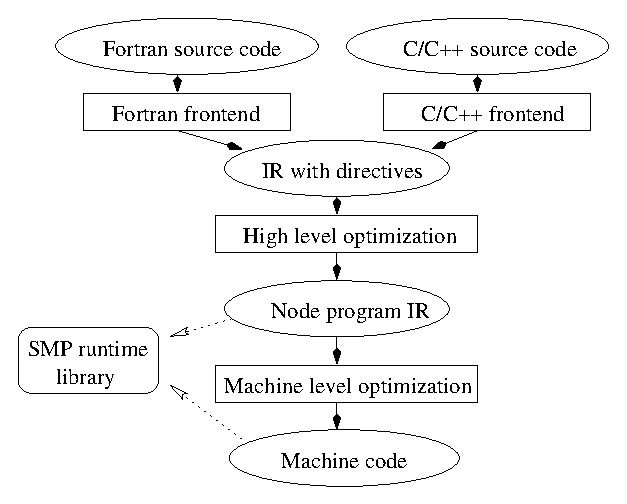
\includegraphics[angle=0, width=0.65\textwidth]{runtime.eps}
    \caption{\footnotesize Compile and runtime environment}
    \label{fig:runtime}
  \end{center}
\end{figure}


\begin{figure}[h!]
  \begin{center}
    % run boxfill.pl to get the filled version of the graph
    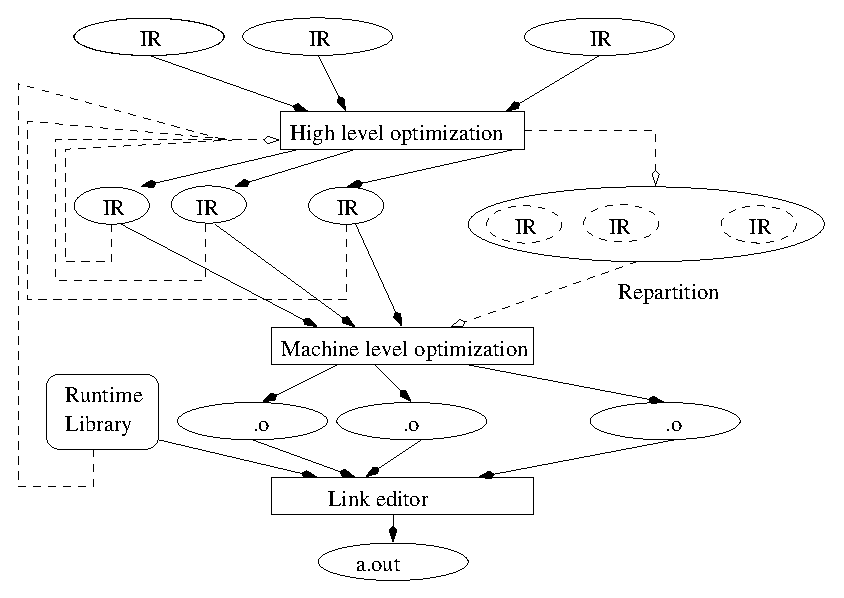
\includegraphics[angle=0, width=0.8\textwidth]{linkphase.eps}
    \caption{\footnotesize Compile and link phase optimization}
    \label{fig:linkphase}
  \end{center}
\end{figure}

SPEC2000 CPU benchmark suite was used to evaluate our techniques, as
it is one of the best indicators of the performance of the processor,
memory and compiler. Our tests focus on Spec2000FP, considering that
it is where most of the data parallel processing exists. The hardware
system used for testing in this paper is 1.1GHz POWER4\textsuperscript \texttrademark system, with 1
to 8 nodes available.

\subsection{Basic Parallelizer Structure}


{\small
\begin{algorithm}[h]
%  \SetLine %this is for setting vertical line with keyword end
  \SetKw{KwBreak}{break}
  \SetKw{KwContinue}{continue}
  \SetKwInOut{Input}{Input}
  \SetKwInOut{Output}{Output}
%  \Input{A desired loop permutation order $O=(L_1,L_2,...,L_n)$, \\
%    the original dependence matrix $\mathcal{D}$ for the loop}
%  \Output{A nearby permutation $P$}
  \BlankLine

  \Begin {
    \For {each loop nest in a procedure} {
      \For {each loop in the nest in the reverse depthfirst order (outer first)} {
        \If {the loop is user parallel} {
          \KwBreak
        }
        
        \If {the loop is marked sequential, has side-effects etc} {
          \KwContinue
        }
        
        \If {the loop has loop carried dependence} {
           try splitting the loop to eliminate dependence
           
           \If {dependence not eliminated}{
               \KwContinue
           }
        }
      
        \If {loop cost is known at compile time} {
          \If { the loop has not enough cost }
             \KwBreak
        }
        \Else {
          Insert code for run-time cost estimate
        }
        Mark this loop auto parallel \\
        \KwBreak
      }
    }
  }
  \caption{Basic loop parallelizer}
  \label{alg:parallelizer}
\end{algorithm}
}

Dependence analysis is a core part of the parallelizer. Data
\emph{dependence vectors}\cite{Ban88} are still our principal tools to
analyze and verify the transformation applied on a loop nest. Suppose
$\vec{\delta} =\{\delta_{1}\dots\delta_{n}\}$ is a hybrid
distance/direction vector with the most precise information derivable.

If we have

%It represents a \emph{data dependence} between two
%array references, corresponding left to right from the outermost loop
%to innermost loop enclosing the references. Data dependences are
%\emph{loop-independent} if the accesses to the same memory location
%occur in the same loop iteration; they are \emph{loop-carried} if the
%accesses occur on different loop iterations.


{\small
\begin{alltt}
\(L\sb{1}\)   DO i\(\sb{1}\) = 1, U\(\sb{1}\)
\(L\sb{2}\)     DO i\(\sb{2}\) = 1, U\(\sb{2}\)
         \dots
\(L\sb{n}\)       DO i\(\sb{n}\) = 1, U\(\sb{n}\)
\(S\sb{1}\)         A(\(f\sb{1}\)(i\(\sb{1}\),\(\dots\),i\(\sb{n}\)),\(\dots\),\(f\sb{m}\)(i\(\sb{1}\),\(\dots\),i\(\sb{n}\)))=\(\cdots\)
\(S\sb{2}\)         \(\cdots\)=A(\(g\sb{1}\)(i\(\sb{1}\),\(\dots\),i\(\sb{n}\)),\(\dots\),\(g\sb{m}\)(i\(\sb{1}\),\(\dots\),i\(\sb{n}\)))
\(T\sb{1}\)         B(\(u\sb{1}\)(i\(\sb{1}\),\(\dots\),i\(\sb{n}\)),\(\dots\),\(u\sb{m}\)(i\(\sb{1}\),\(\dots\),i\(\sb{n}\)))=\(\cdots\)
\(T\sb{2}\)         \(\cdots\)=B(\(v\sb{1}\)(i\(\sb{1}\),\(\dots\),i\(\sb{n}\)),\(\dots\),\(v\sb{m}\)(i\(\sb{1}\),\(\dots\),i\(\sb{n}\)))
         END DO
         \dots
       END DO
     END DO
\end{alltt}
}

as a loop nest from $L_{1}$ to $L_{n}$, we may have two dependences
$\vec{\delta}_{A}$ and $\vec{\delta}_{B}$ characterizing the nested
loops, which were caused by $S\sb{1}$/$S\sb{2}$ and
$T\sb{1}$/$T\sb{2}$, where $f$, $g$, $u$, $v$ are linear functions of
the loop induction variables. \emph{Dependence matrix}, denoted as $\mathcal{D}$, includes
$\vec{\delta}_{A}$ and $\vec{\delta}_{B}$ as two rows.

The Algorithm \ref{alg:parallelizer} shows the basic structure of the
parallelizer. The parallelizer scans through all the loop nests in a procedure
looking for parallelizable loops.  Nested parallelism is avoided by
parallelizing only one loop in every nest.  The loops in a nest are
scanned from outer to inner as outer loops have a greater benefit from
parallelization than inner loops. As a first step, loops that are not normalized and loops that are explicitly marked as sequential or have residuals, side-affects or with loop carried dependences are discarded by the parallelizer at compile time. For loops with loop carried dependences, the parallelizer tries to split the loop to eliminate the dependences. The loops are then parallelized independently. This preliminary step eliminates all non-parallelizable loops. However, naively executing all the parallelizable loops in an application may not be a good idea as we will soon discover. Parallelization is a very expensive operation with high overhead and the compiler has to be very judicial in identifying loops that can benefit from parallelization. 

This paper omits discussions about basic techniques of computing dependence matrix, privatizing scalar variables in a
loop, finding reduction variables, peeling or splitting the loop to
eliminate the loop carried dependence, etc. which are all parts of the preparation
phase for the parallelizer. We focus instead on the advanced techniques used by the parallelizer to intelligently select loops for parallelization and the optimizations that can be done after identifying a parallelizable loop. Section \ref{selection} deals with loop transformation techniques that can enhance the parallel performance of loops selected for parallelization. Section \ref{cost} explores the use of loop cost as an advanced loop selection technique for parallelization. 


%\newpage

\section{Balancing coarse-grained parallelism and locality}
\label{selection}

There are many loop transformation techniques that exists today\cite{All02}. And almost all of them can be applied to more than
one kind of code optimizations. For example, loop interchange is
widely used to improve data locality in cache management. Meanwhile, it
also can be used to exploit parallelism, such as vectorization, and
even coarse-grained parallelism.  Unfortunately, the transformations
for different optimization purposes do not always work in harmony.

For instance, in a loop nest, maximum spatial cache reuse can be achieved by moving the loop with stride-one access of the references to the innermost position. So a loop permutation
algorithm will try to calculate such a loop order while keeping the
dependence constraints of the original loop nest. On the other hand, in an automatic parallelizing compiler, one would
like to parallelize the outermost loop to reduce the parallel region
setup overhead, and leave more code in the inner loop for other
optimization opportunities. 

There has been significant research to study different approaches to solve this problem.
A well known technique is \emph{Unimodular transformation}
\cite{Mic91,Lam91,Ban90}, a compound loop transformation algorithm aiming at
integrating different loop transformations for a specific goal and
target machine, thereby reducing the problem of finding the best
transformation combination to finding the best unimodular matrix. Another technique is \emph{Loop selection}\cite{All02}, which
parallelizes all the parallelizable loops, then uses heuristics to
select the next one as sequential, expecting to find more
parallelizable loops after that. This is easier to implement when compared to
unimodular transformation.

Our work is based on the idea of loop selection, but is different from
the original one in two aspects: a) given our target is an OpenMP node
program, we only need to find one parallelizable loop per nest, to avoid
generating code with nested parallelism; b) our heuristics are
directly linked to data locality, unlike the original loop selection
technique which picks a loop with most ``$<$'' directions to parallelize.

\subsection{Analyzing model}

Using the notation in Section \ref{par_structure}, we introduce two
theorems.

\begin{theorem}[C-level interchangeable] \label{theorem:interchange}
  Loop $L_{c}$ and $L_{c-1}$ is interchangeable if and only if   
   $\forall \vec{\delta} \in \mathcal{D}$, $\vec{\delta} \neq
  (=^{(c-2)} < > \ldots)$, where ``$=^{(c-2)}$'' indicates that there are
  $(c-2)$ directions as ``$=$'' before the first ``$<$''.
\end{theorem} 

Theorem \ref{theorem:interchange} and its variant forms can be found
in \cite{Zim90} and other literatures. We will not prove it here, but 
use it directly for our theorem later.

\begin{theorem}[P-level parallelizable] \label{theorem:parallelize}
  Loop $L_{p}$ can be parallelized as a parallel do if and only if
   $\forall \vec{\delta} \in \mathcal{D}$, $\vec{\delta} \neq
  (=^{(p-1)} < \ldots)$.
%, where ``$=^{(p-1)}$'' means there are $(p-1)$
%  directions as ``$=$'' before the first ``$<$''.
\end{theorem} 

The proof for Theorem \ref{theorem:parallelize} is trivial. By the
definition of parallel do, it cannot carry any dependence.

Next, we define a \emph{multiply} operation on a dependence vector.
Let $ \vec\sigma=\vec{\sigma}_{a} \times \vec{\sigma}_{b}$, where
$\forall \sigma_{j} \in \vec\sigma, \sigma_{j} = \sigma_{a_{j}} \times
\sigma_{b_{j}}$. The multiplication of the two dependence distances is
defined as following. It is unknown if one of the distances is unknown.
Otherwise, it will be the regular multiplication on two integers. If
one of the distances is only a direction, it is treated as 1 or -1, and
after the multiplication, converted back to a direction .

Let $\vec{\sigma}_{p}$ and $\vec{\sigma}_{p-1}$ be the $p^{th}$,
$(p-1)^{th}$ column vector of dependence matrix $\mathcal{D}$, then we
have

\begin{theorem}[Keeping it parallelizable] \label{theorem:keep}
  A p-level parallelizable loop $L_{p}$ can be interchanged to
  $L_{p-1}$ and becomes (p-1)-level parallelizable if and only if 
  $\forall \sigma_{j} \in \vec{\sigma}$, where $\vec{\sigma} =
  \vec{\sigma}_{p-1} \times \vec{\sigma}_{p}$, either
  \begin{itemize}
  \item $\sigma_{j}=0$ or 
  \item the $j^{th}$ dependence in $\mathcal{D}$ is not carried by
    $L_{p-1}$
  \end{itemize}
\end{theorem} 

\begin{flushleft}
\textbf{Proof} 
\end{flushleft}

We start by proving the ``\emph{if}'' part of the theorem.

Suppose $\forall \sigma_{j}=0$. 

First, we can assert that $L_{p-1}$ and
$L_{p}$ is interchangeable. Otherwise, according to Theorem
\ref{theorem:interchange} there is a dependence vector $\vec{\delta}$
that has the form of $(=^{(p-2)} < > \ldots)$. This will conflict with the
fact that all $\sigma_{j}$ is zero.
Secondly, we prove that the $L_{p}$ will become $(p-1)$-level
parallelizable after interchanging with $L_{p-1}$.  Otherwise, from
Theorem \ref{theorem:parallelize}, there will a dependence vector
$\vec{\delta}$, of the format $(=^{(p-2)} < \ldots)$, in the
dependence matrix preventing it from being parallelized after the
interchange. Considering the format of the $\vec{\delta}$ before the
interchange, given that all $\sigma_{j}$ is zero, it should be in the
form of $(=^{(p-1)} < \ldots)$. This conflicts with the fact that $L_{p}$
is parallelizable according to Theorem \ref{theorem:parallelize}.

If $\exists \sigma_{j} \neq 0$, we let $\vec{\delta}$ be the
dependence vector on the $j^{th}$ row of the matrix. It should have
one of the following formats $(\cdots^{(p-2)} < < \ldots)$,
$(\cdots^{(p-2)} < > \ldots)$, $(\cdots^{(p-2)} > < \ldots)$,
$(\cdots^{(p-2)} > > \ldots)$, where $\cdots^{(p-2)}$ is the leading
$(p-2)$ positions. Since $L_{p-1}$ does not carry any dependences as
in the given condition, $\cdots^{(p-2)}$ has to be in the format of
$(= \ldots = < \ldots)$, in order for the $\delta$ to be valid. Therefore,
$L_{p}$ can be interchanged with $L_{p-1}$ and still be kept parallelizable.

Similarly, the ``\emph{only if}'' part of the theorem can be proved. This is not important in our algorithm, so we will omit it here.

\begin{flushright}
\textbf{End of Proof} 
\end{flushright}

\begin{theorem}[Outermost parallelizable] \label{theorem:outermost}
  Loop $L_{o}$ can be parallelized at the outermost level if and only
  if  $\vec{\sigma} = \vec{0}$, where $\vec{\sigma}$ is the
  $o^{th}$ column vector of dependence matrix $\mathcal{D}$.
\end{theorem} 

This is a direct conclusion from Theorem \ref{theorem:keep}. It is
actually used in \cite{All02} for loop selection.

\subsection{Loop permutation with examples}
\label{sec:algorithms}


%{\small
%\begin{algorithm}[h]
%%  \SetLine %this is for setting vertical line with keyword end
%  \SetKw{KwBreak}{break}
%  \SetKwInOut{Input}{Input}
%  \SetKwInOut{Output}{Output}
%  \Input{A desired loop permutation order $O=(L_1,L_2,...,L_n)$, \\
%    the original dependence matrix $\mathcal{D}$ for the loop}
%  \Output{A nearby permutation $P$}
%  \BlankLine

%  \Begin {
%    \If{$\forall \delta \in \mathcal{D}$, $O$ is legal}{
%      \KwRet $O$ \;
%    }
%    $P:=\emptyset$; $k:=0$; $m:=n$\;
%    \While{$O \neq \emptyset$} {
%      \For{$i:=1$ \KwTo $m$} {
%        \If {$\forall \delta, (P_1,...,P_k, L_i)$ is legal} {
%          $P:=(P_1,...,P_k, L_i)$ \;
%          $O:=O-\{L_i\}$\; 
%          $k:=k+1$; $m:=m-1$ \;
%          \KwBreak
%        }
%%        select the leftmost loop $l$ in $O$ \\
%%        such that $(P_1,P_2,...,P_{i-1},l)$ has no illegal direction vector prefixes \;
%%        remove $l$ from $O$ \;
%%        append $l$ to the end of $P$, so that it becomes $P_i$ \;
%      }
%    }
%  }
%  \caption{Select a permutation for data locality}
%  \label{alg:permutelocal}
%\end{algorithm}
%}

Based on our discussion in the previous section, we try to find a
permutation favoring both data locality and parallelism. To do this, 
we first assign each loop induction variable with a weight in terms
of memory access. We will favor those having maximum memory spatial
reuse.  A more comprehensive way of evaluating the weights is called
profitability-based methods, introduced in \cite{All02}, which has a
cache model to estimate cache misses. Either way, a memory ordering
$O=(L_1,L_2,...,L_n)$ of the nested loops is calculated, where $L_1$
has the least reuse and $L_n$ the most.

Next we build up a nearby legal permutation in $P$ by first testing to see if the loop $L_1$ is
legal in the outermost position.  If it is legal, it is added to $P$
and removed from $O$. If it is not legal, the next loop in $O$ is
tested.  Once a loop $L_{i}$ is positioned, the process is repeated
starting from the beginning of $O-\{L_{i}\}$ until $O$ is empty. $P$
is considered as having the best data locality for the loop nest. The algorithm is summarized in \cite{Mck96},

%{\small
%\begin{algorithm}[h]
%%  \dontprintsemicolon
%%  \SetLine %this is for setting vertical line with keyword end
%  \SetKw{KwBreak}{break} 
%  \SetKwInOut{Input}{Input}
%  \SetKwInOut{Output}{Output}
%  \Input{A loop order $O=(L_1,L_2,...,L_n)$ in favor of data locality, \\
%    the original dependence matrix $\mathcal{D}$ for the loop}
%  \Output{A permutation $P$ considering coarse-grained parallelism as
%    well} 
%  \AlgData{two integers $src$, $dst$ to represent preferred move}

%  \BlankLine

%  \Begin {
%    \If{$L_1$ is parallelizable} {
%      \KwRet $O$ \;
%    }
%    $src:=n$; $dst:=n$ \;
%    \For {$i:=2$ \KwTo $n$} {
%      \If {$L_i$ is parallelizable} {
%        \For {$j:=i-1$ \KwTo $1$} {
%          \If {$L_i$ can be moved before $L_j$} {
%            \If {$j < dst$} {
%               $src:=i$; $dst:=j$ \;
%               \lIf{$dst=1$} {\KwBreak}
%            }
%          }
%        }
%        \lIf{$dst=1$} {\KwBreak}
%      }
%    }
%    construct $P$ with $src$ and $dst$ 
%  }
%  \caption{Select a permutation for parallelism}
%  \label{alg:permutepar}
%\end{algorithm}
%}

%Finally, we use Algorithm \ref{alg:permutepar} to do further
%adjustment. Given all the parallelizable loops in the nest, it try to
%move a parallelizable loop outer as much as possible.

Finally, we can adjust the other loops further, based on the
following conditions to decide if $L_i$ can be moved before $L_j$,

\begin{itemize}
\item The interchange should be legal,
\item $L_i$ is still parallelizable after moving, and
\item The amount of data locality we are willing to sacrifice.
\end{itemize}

The first two questions are answered by Theorem \ref{theorem:keep}.
We will use heuristics including the induction variable weights
calculated previously to control how aggressive the parallelizer
should be. Apart from estimating the cache miss, a good heuristic could
also include estimations of the loop cost and parallel setup overhead. The
topics deserve some discussions on their own, and will not be
included here. \emph{Strip-mining} can also be considered, if no
loop can be moved at all.

%We used an XL FORTRAN 8.1 based development compiler on an 8 node
%1.1GHz POWER4 system to do the following test. 

We illustrate the benefits of using our loop permutation algorithm using a simple example. Loop permutation for data locality will transform the Fortran code shown below to \texttt{K} loop as the outermost and \texttt{I} loop as the innermost in the nest. This
will lead to the middle \texttt{J} loop getting parallelized. With our loop
permutation algorithm we can have the \texttt{J} loop moved to the
outermost position, thus striking a balance between locality and the desired coarse-grained parallelism.

{\small
\begin{verbatim}
 DO I = 1, N
   DO J = 1, N
     DO K = 1, N 
       A(I,J,K)=A(I,J,K+1);
     END DO
   END DO
 END DO
\end{verbatim}
}


%{\small
%\begin{verbatim}
% DO K = 1, N
%   DO J = 1, N
%     DO I = 1, N 
%       A(I,J,K)=A(I,J,K+1);
%     END DO
%   END DO
% END DO
%\end{verbatim}
%}

%Since \texttt{I} has stride-one access to the array \texttt{A}, it
%will be moved to the innermost position. If we enable the
%auto-parallelizer, compiler will generate code roughly corresponding
%the following segment,

%{\small
%\begin{verbatim}
%      DO K = 1, N
%!OMP$ PARALLEL DO
%        DO J = 1, N
%          DO I = 1, N
%            A(I,J,K)=A(I,J,K+1);
%          END DO
%        END DO
%      END DO
%\end{verbatim}
%%$ closing dolar
%}

%With Algorithm \ref{alg:permutepar} implemented, the final results can
%be further improved as,

%{\small
%\begin{verbatim}
%!OMP$ PARALLEL DO
%      DO J = 1, N
%        DO K = 1, N
%          DO I = 1, N 
%            A(I,J,K)=A(I,J,K+1);
%          END DO
%        END DO
%      END DO
%\end{verbatim}
%%$ closing dolar
%}

\begin{figure}[!t]
  \begin{center}
    % run boxfill.pl to get the filled version of the graph
    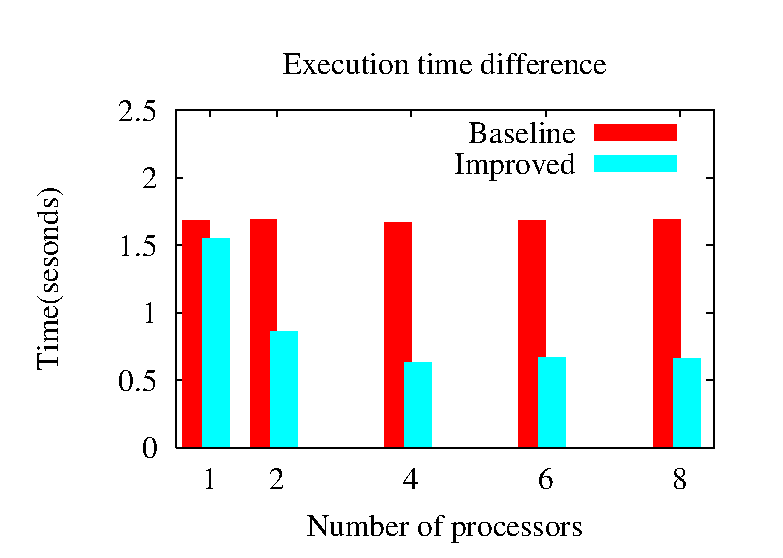
\includegraphics[angle=0, width=0.55\textwidth]{compare.eps}
    \caption{\footnotesize Performance difference}
    \label{fig:compare}
  \end{center}
\end{figure}

Figure \ref{fig:compare} shows the performance difference of the
generated code on the POWER4 system for both the cases discussed. \texttt{N} is set to 100 and the loop nest is executed 100 times. In the figure, ``Baseline'' and
``Improved'' use exactly the same compiler, with the only difference being that the parallel loop
is in the middle for the ``Baseline'' case and the outermost for the ``Improved'' case. We can see that the parallel setup overhead completely offsets the gain from parallelization in the first case,
while the improved version sees reasonable speedup even for a loop with 
small computation cost (the loop body has a single assignment statement).

In the SPEC2000FP suite, \texttt{mgrid} was negatively affected by this
transformation, further experiments are being carried out to derive better heuristics.

%\newpage

\section{Restricting parallelization using cost estimation}
\label{cost}

After a preliminary filtering out of loops unsuitable for
parallelization using Algorithm~\ref{alg:parallelizer}, the
auto-parallelizer evaluates the cost of a loop to further refine the
selection of parallel loops. 

\subsection{Loop Cost Model}
The
cost of a loop is the approximate execution time of the loop and is
given by 

{\small
\begin{displaymath}
       LoopCost = (IterationCount * ExecutionTimeOfLoopBody)
\end{displaymath}
}
The loop cost algorithm is a recursive algorithm that computes the
approximate execution time of the loop including all nested loops
inside the current loop. To evaluate loops based on the loop cost, we
define a set of \emph{Threshold} values as the basis for comparison.
The threshold values are carefully chosen values based on heuristics
and take into account the number of processors, overhead arising from
the setup required for parallelization, etc.

For loops whose cost can be estimated at compile-time, the parallelizer
simply compares the cost against the precomputed threshold value and
rejects loops with low costs. However for loops whose cost cannot be
determined at compile-time (which is mostly the case), the
auto-parallelizer computes a cost expression for the loop in terms of the
values known only at runtime. This expression is then evaluated at
runtime to determine whether the loop is worth parallelizing. The
runtime cost expression is kept as lightweight as possible because of
the overhead incurred in computing the expression at runtime. The
auto-parallelizer also has a mechanism to limit the number of threads
used to parallelize a loop depending on the cost of the loop.
Table~\ref{autopar_loops} shows the parallel loops selected at
different stages of filtering.

Figure ~\ref{fig:loopcost_performance} shows the effectiveness of using the
Loop Cost Model to restrict parallelization. The results show that
careful restriction and appropriate selection of loops for
parallelization is extremely crucial for parallel performance.
Evaluation of our auto-parallelization techniques for Spec2000FP
benchmarks indicate that the auto-parallelizer is quite precise in
selecting high-cost loops for parallelization as shown by
Table~\ref{autopar_accuracy}. The Spec2000FP benchmarks were analyzed
using Profile Directed Feedback techniques \cite{Cohn99} \cite{Sch98}
to identify the high-cost loops in the program. The loops selected by
the auto-parallelizer are then compared with the list of expensive
loops obtained from profile directed feedback. From
Table~\ref{autopar_accuracy} we can see that the auto-parallelizer is
quite accurate within a small error margin.  Column 4 of
Table~\ref{autopar_accuracy} indicates the number of loops incorrectly
picked by the parallelizer, i.e., loops that have a low cost and hence are not
worth parallelizing. It is important to keep this number a minimum as
selecting the wrong loop can adversely impact the parallel execution
performance. The zero values in Column 4 indicate that the
parallelizer never picks the wrong loops.


\begin{figure}[h!]
  \begin{center}
    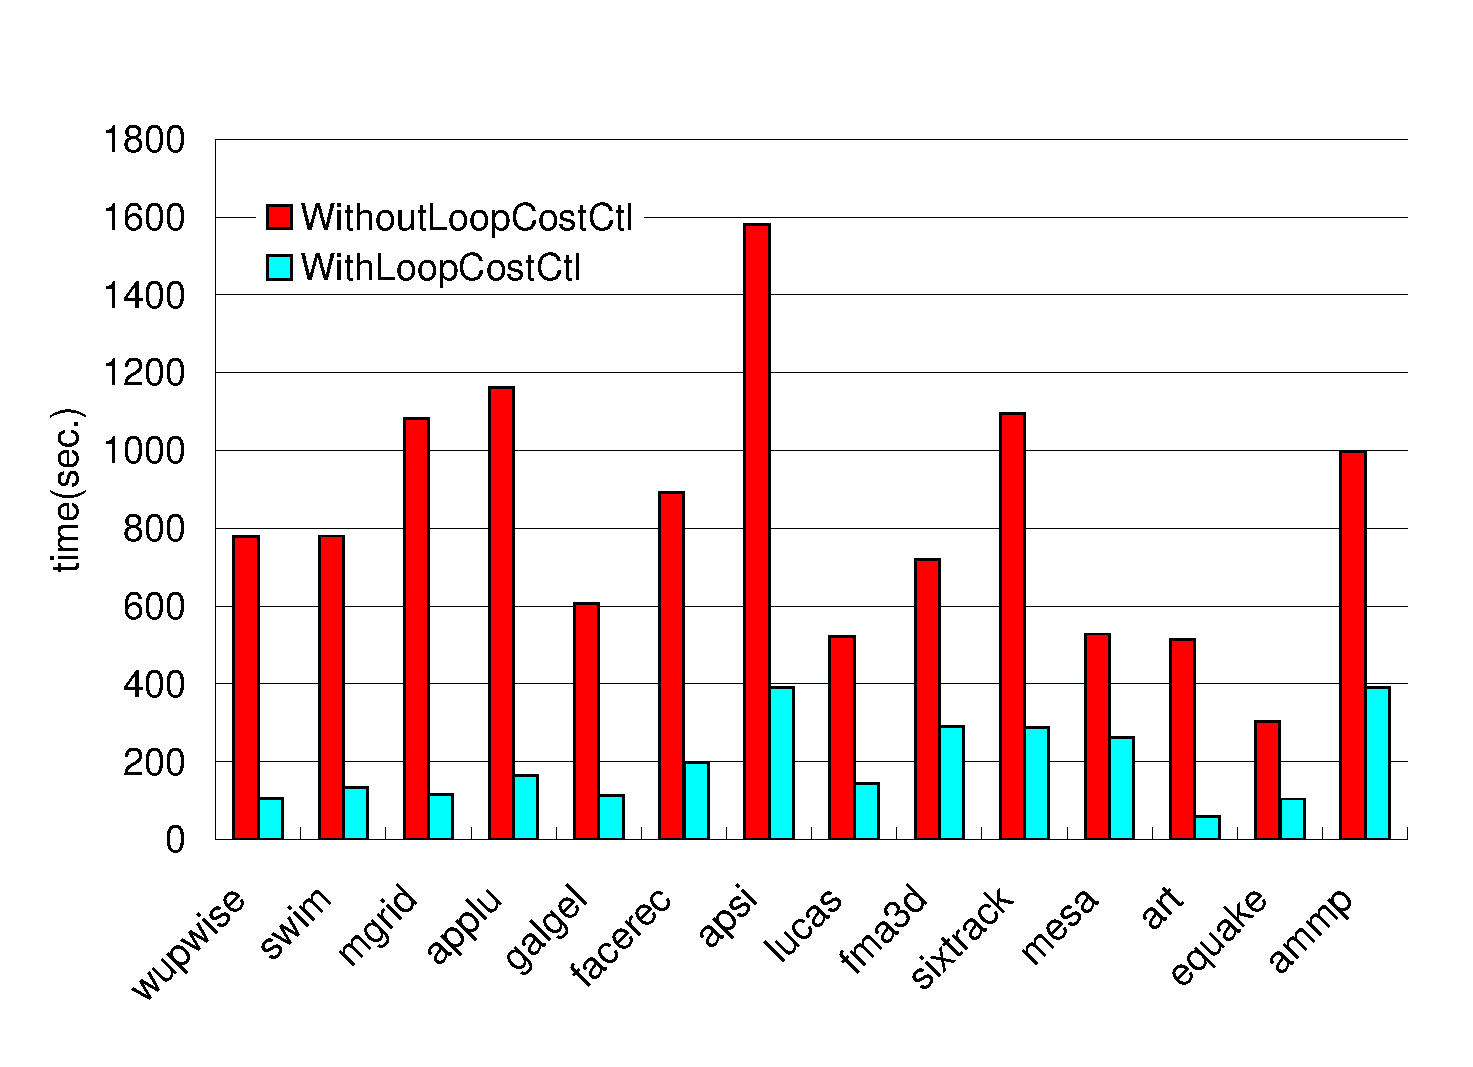
\includegraphics[angle=0, width=0.85\textwidth]{loopcost.eps}
    \caption{\footnotesize Benchmark performance with and without Loop Cost using two CPU's}
    \label{fig:loopcost_performance}
  \end{center}
\end{figure}


%\begin{table}
%\begin{center}
%\begin{tabular}{|l|c|c|} \hline
%\bf Benchmark & \bf Time(sec) & \bf Time(sec)\\
%& \bf Without Loop Cost & \bf With Loop Cost  \\
%\hline
%\hline
%swim & 780.18 & 134.56 \\ 
%\hline
%wupwise & 778.61 & 104.28 \\ 
%\hline
%mgrid & 1081.24 & 116.36\\
%\hline
%applu & 1161.56 & 163.92\\
%\hline
%galgel & 605.53 & 112.05\\
%\hline
%lucas & 522.34 & 142.92\\
%\hline
%mesa & 548.24 & 263.27\\
%\hline
%art & 513.68 & 60.10\\
%\hline
%equake & 302.97 & 103.98\\ 
%\hline
%ammp & 997.50 & 391.81 \\
%\hline
%apsi & 1581.05 & 390.63 \\
%\hline
%sixtrack & 1095.94 & 286.96 \\
%\hline
%fma3d & 720.80 & 291.52 \\
%\hline
%facerec & 891.11 & 196.63 \\
%\hline
%\end{tabular}
%\vspace{0.5cm}
%\caption{\label{loopcost_performance}Benchmark performance with and without Loop Cost}
%\end{center}
%\end{table}

% Enclosing tabular in a table ...compacts the table ie reduces the spacing between rows. It becomes Floating tables
\begin{table}
\begin{center}
\begin{tabular}{|l|c|c|c|c|c|} \hline
{\rule[-2mm]{0mm}{6mm}\bf Benchmark} & \bf \#Input Loops & \bf \#Loops Processed & \bf \#After Stage1 & \bf \#After Stage2/ & \bf\#After Stage3 \\
\hline
\multicolumn{6}{|c|}{\bf Stage1: Preliminary compile-time filtering }\\
\multicolumn{6}{|c|}{\bf Stage2: Compile-time loop cost filtering  }\\
\multicolumn{6}{|c|}{\bf Stage3: Runtime loop cost filtering  }\\
\hline
\hline
swim & 23 & 18 & 9 & 9 & 5\\
\hline
wupwise & 58 & 58 & 6 & 6 & 4\\ 
\hline
mgrid & 47 & 30 & 11 & 11 & 7\\ 
\hline
applu & 180 & 104 & 27 & 27 & 11\\ 
\hline
galgel & 642 & 538 & 280 & 280 & 36\\ 
\hline
lucas & 123 & 123 & 16 & 16 & 4\\ 
\hline
mesa & 777 & 777 & 118 & 118 & 0\\ 
\hline
art & 83 & 83 & 18 & 18 & 5\\ 
\hline
equake & 62 & 64 &  0 & 0 & 0\\ 
\hline
ammp & 283 & 282 & 18 & 18 & 0\\ 
\hline
apsi & 303 & 284 & 92 & 92 & 5\\ 
\hline
sixtrack & 1157 & 1135 & 347 & 347  & 11 \\ 
\hline
fma3d & 1648 & 1635 & 272 & 272 & 33\\ 
\hline
facerec & 202 & 133 & 69 & 69 & 9\\ 
\hline
\end{tabular}
\vspace{0.5cm}
\caption{\label{autopar_loops}Stages of Loop Selection for Auto-parallelization of Spec2000 FP Benchmarks}
\end{center}
\end{table}

\begin{table}
\begin{center}
\begin{tabular}{|l|c|c|c|c|} \hline
\bf Benchmark & \bf \#HighCostLoops & \bf \#Parallelizable & \bf \#HighCostLoops & \bf \#LowCostLoops \\
& \bf from PDF & \bf HighCostLoops& \bf selected by & \bf  selected by \\
& & \bf from PDF & \bf Parallelizer & \bf Parallelizer \\
\hline
\hline
swim & 8 & 5 & 5 & 0 \\
\hline
wupwise & 7 & 4 & 4 & 0 \\ 
\hline
mgrid & 9 & 7 & 7 & 0\\ 
\hline
applu & 41 & 11 & 11 & 0 \\ 
\hline
galgel & 84 & 49 & 36 & 0 \\ 
\hline
lucas & 47 & 4 & 4 & 0 \\ 
\hline
mesa & 74 & 3 & 0 & 0 \\ 
\hline
art & 37 & 5 & 5 & 0 \\ 
\hline
equake & 8 & 0 & 0 & 0 \\ 
\hline
ammp & 31 & 0 & 0 & 0 \\ 
\hline
apsi & 28 & 11 & 5 & 0 \\ 
\hline
sixtrack & 44 & 13 & 11 & 0 \\ 
\hline
fma3d & 61 & 33 & 33 & 0 \\ 
\hline
facerec & 43 & 25 & 9 & 0 \\ 
\hline
\end{tabular}
\vspace{0.5cm}
\caption{\label{autopar_accuracy}Evaluation of Loop Selection for Auto-parallelization of Spec2000 FP Benchmarks}
\end{center}
\end{table}

\subsection{Runtime Profiling}

In addition to using loop cost for restricting parallel loops, the auto-parallelizer employs runtime profiling\cite{Nan03} to further filter out
loops at a finer granularity. The runtime profiling is a more accurate
way of measuring the execution time of a chunk of code. The execution
time of a chunk of a loop executed in parallel (as measured by the
runtime profiler) is compared with selected \emph{serial} and
\emph{parallel} thresholds. If the execution time of the chunk is less
than the serial threshold, the next chunk of the loop is serialized
disregarding the decision from the runtime loop cost evaluation. The
decision to parallelize or serialize changes dynamically depending on
previous executions of the loop.




%\newpage

\section{Missed parallelization opportunities}
\label{opportunities}

As expected, the performance improvements from auto-parallelization
are limited (refer to Section \ref{summary} for the actual data). To understand the auto-parallelization results, we compare our results with the SPECOMP benchmarks. For an SMP machine with a small number of processors, SPECOMP achieves relatively good performance and scalability. With this comparison, we hope to understand the reasons for the disparity in the results between explicit and auto parallelization and also expose opportunities missed by the auto-parallelizer.

Among the 14 SPEC2000FP benchmarks, 10 of them are also included in
SPECOMP test suite. The two versions of the benchmarks were compared on a loop-to-loop basis. This analysis exposes limitations in the auto-parallelizer and also led to some very interesting observations. We list here some of the cases where the auto-parallelizer failed to parallelize a loop that was explicitly parallelized in the SPECOMP version. We believe that improvements to the auto-parallelizer to handle these cases can result in significant performance
improvements for at least some of the benchmarks. To prove this, we try to manually parallelize loops that were explicitly parallelized in SPECOMP and compare the performance gain (manual parallelization is not possible in all cases).
 

\subsection {Case 1: Loop body contains function calls}

The auto-parallelizer fails to parallelize loops that have function calls in the loop body. Function calls could result in side-effects; the current auto-parallelizer is not capable of handling such loops. 
Shown here is a code snip found in \emph{wupwise} where the loop body has function calls. \emph{wupwise} has four such case, two in muldeo.f and
 two in muldoe.f. Manual parallelization of such loops shows good speedup. To manually parallelize the loops, array's AUX1 and AUX3 were privatized. The execution time is about 114 seconds with one thread, 61.8 seconds for
two threads and 46.5 seconds with four threads, i.e., a 46\% improvement with 2 threads and 59\% improvement with 4 threads over using 1 thread. More complicated forms of this case exists in \emph{apsi}, \emph{galgel} and \emph{applu}

{\small
\begin{verbatim}
      COMPLEX*16   AUX1(12),AUX3(12)
      ....
      
      DO 100 JKL = 0, N2 * N3 * N4 - 1
        L = MOD (JKL / (N2 * N3), N4) + 1
        LP=MOD(L,N4)+1
        K = MOD (JKL / N2, N3) + 1
        KP=MOD(K,N3)+1
        J = MOD (JKL, N2) + 1
        JP=MOD(J,N2)+1
        DO 100 I=(MOD(J+K+L,2)+1),N1,2
          IP=MOD(I,N1)+1
          CALL GAMMUL(1,0,X(1,(IP+1)/2,J,K,L),AUX1)
          CALL SU3MUL(U(1,1,1,I,J,K,L),'N',AUX1,AUX3)
          CALL ZCOPY(12,AUX3,1,RESULT(1,(I+1)/2,J,K,L),1)
100   CONTINUE
\end{verbatim}
}

\subsection {Case 2: Array privatization}

Several loops in SPECOMP benchmarks have arrays that are explicitly marked as private, enabling the loops to be parallelized. Array privatization analysis is not yet implemented in our parallelizer preventing it from exploiting these opportunities. The code snip in Case 1 illustrates an example where array privatization is required in order to parallelize the loop. 3 such nested loops can be found in subroutine \emph{rhs} of \emph{applu}. Manual parallelization of such loops resulted in a 12\% performance gain for \emph{applu}. Similar situations exist in \emph{galgel} and {apsi}

\subsection{Case 3: Zero trip loops}

Zero trip loops are loops in which the number of iterations calculated
from the parameters of the loop is less than 1. There are 8 such
loops in \emph{apsi}, one of which is shown below. There exists loop carried dependence on the induction variable L, which the compiler tries to eliminate by rewriting the induction variable in terms of the loop parameters. However, in the case shown here, the parallelizer cannot identify L as an induction variable because of the possibility that the value of NX or NY is zero, thereby preventing the outer loop from getting parallelized. By manually parallelizing the outermost
loop of such loops, the performance of \emph{apsi} was improved by 3\%.

{\small
\begin{verbatim}
      DO 30 K=1,NZTOP
        DO 20 J=1,NY
          DO 10 I=1,NX
            L=L+1
            DCDX(L)=-(UX(L)+UM(K))*DCDX(L)-(VY(L)+VM(K))*DCDY(L)
     *              +Q(L)
 10       CONTINUE
 20     CONTINUE
 30   CONTINUE
\end{verbatim}
}

%\subsection{Pointer used in the loop body}

%There are total 6 loops in the file rectmm.c are parallelized in
%specomp2001 benchmark ammp. The similarity of the loops is that the
%pointer variable pointing to an array or struct is used in the loop
%body. Figure 5 is the code segment from ammp. In the figure, nodelist
%is a pointer to a construct MMNODE. The alias analysis failed to
%eliminate the loop carried dependence of the pointer variables. So the
%parallelizer cannot parallelize the outermost loops. Making these
%loops parallelized would give ammp 7\% performance improvement.


%{\small
%\begin{verbatim}
%  MMNODE (*nodelistt)[];
%  for( ix=0; ix< nx; ix++)
%    for( iy=0; iy< ny; iy++)
%      for( iz=0; iz< nz; iz++)
%        {
%          inode = ((iz*ny)+iy)*nx + ix;
%          (*nodelist)[inode].xc = ix*mmbox + .5*mmbox + xmin;
%          (*nodelist)[inode].yc = iy*mmbox + .5*mmbox + ymin;
%          (*nodelist)[inode].zc = iz*mmbox + .5*mmbox + zmin;
%        }
%\end{verbatim}
%}




\section{Summary and future work} 
\label{summary}

We measured the performance of both the sequential and the auto-parallel versions of SPEC2000FP benchmarks. The results are shown in Figure~\ref{fig:performance}\footnote{The numbers shown here are based
  on a snap shot of our development compiler.}.The figure shows three execution times for each benchmark,
\begin{itemize}
\item \emph{Sequential} : sequential execution time of the benchmark code compiled by our compiler at the highest
optimization level.
\item \emph{Parallel} : parallel (2 threads) execution time of the benchmark parallelized by the auto-parallelizer for SMP machines.
\item \emph{Improved} : parallel (2 threads) execution time with manual changes to the source code as described in Section \ref{opportunities}
\end{itemize}

\begin{figure}[h!]
  \begin{center}
    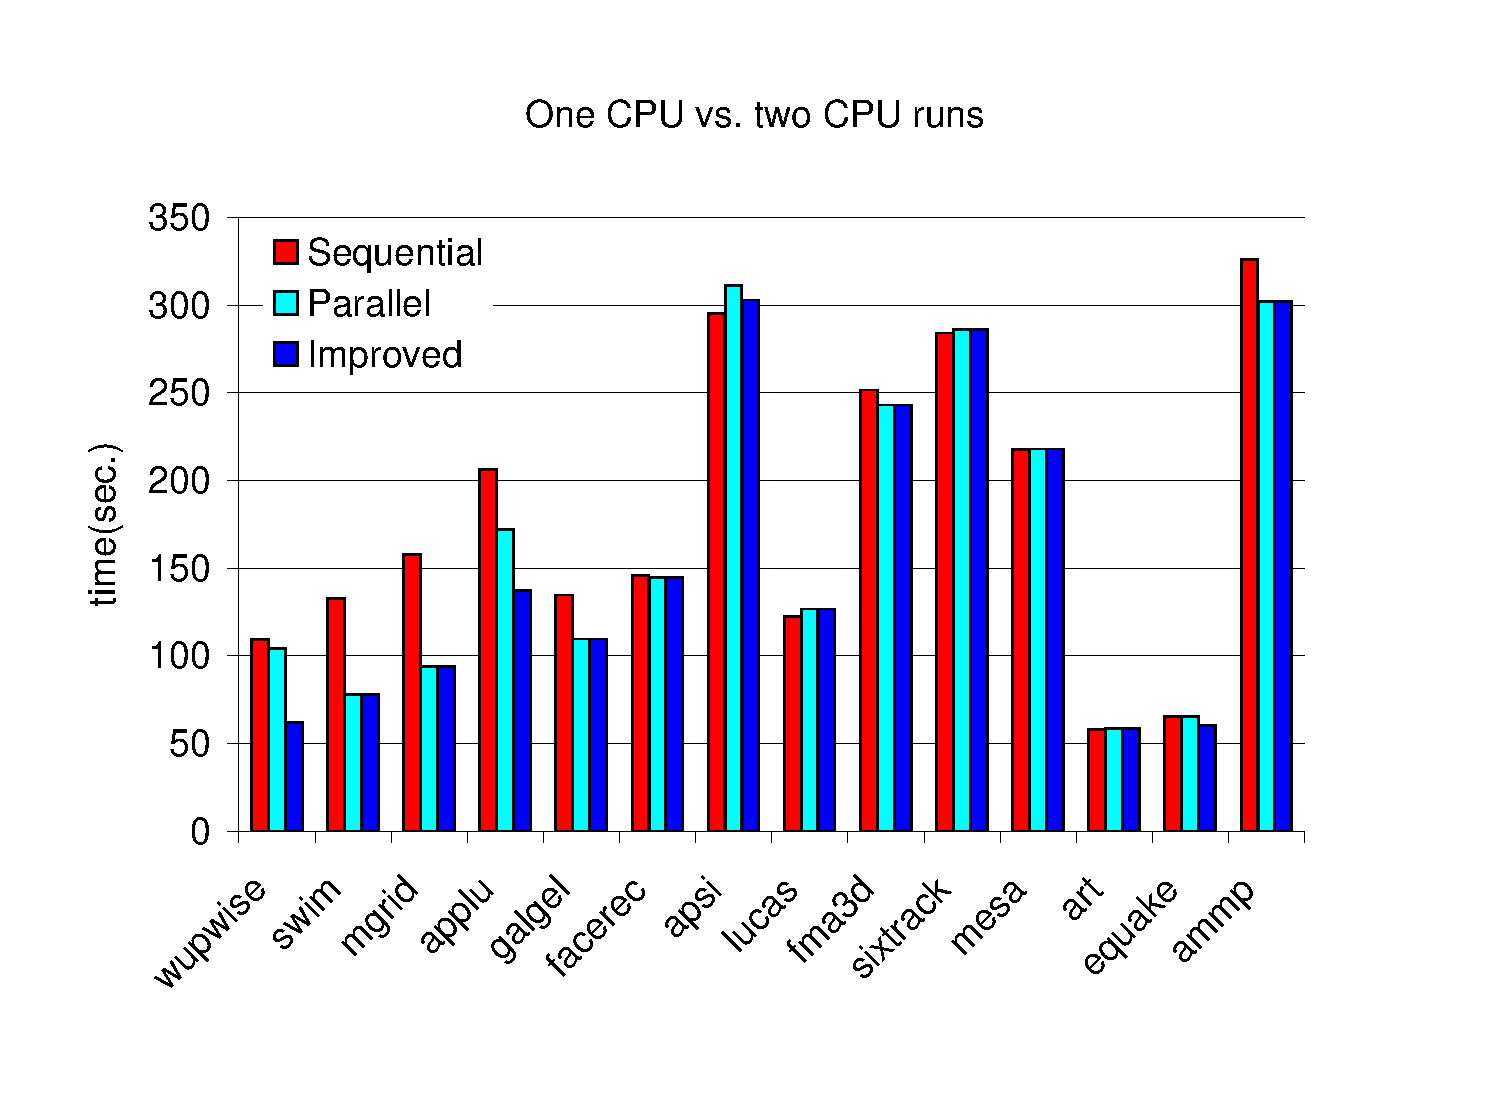
\includegraphics[angle=0, width=0.85\textwidth]{spec2kfp.eps}
    \caption{\footnotesize Performance of auto-parallelization}
    \label{fig:performance}
  \end{center}
\end{figure}

We also emphasize that for simplicity, the modification to individual benchmarks for the \emph{Improved} results address only one specific problem among the 3 identified in Section \ref{opportunities}. For instance, \texttt{apsi} 
is affected by zero trip loops, function calls in the loop body as well as array privatization. However, the source modification includes only source changes for zero trip loops. Among those 10 benchmarks in the SPECOMP test suite, \texttt{swim}, \texttt{mgrid}, \texttt{applu}, \texttt{galgel} and \texttt{wupwise}
see reasonable speedup, with improvement up to 40\%.

The results from auto-parallelization as shown by Figure ~\ref{fig:performance} are not very impressive, especially considering that the hardware resource has actually doubled. However, we argue that the focus in this paper has been the utilization of simple techniques to achieve parallelization with minimal impact on the compilation time. This paper has also shown that much better performance is obtainable using sophisticated techniques at the cost of increased compilation time. In addition, this paper also presents a simple loop permutation algorithm to balance data
locality and coarse-grained parallelism on SMP machines.


Our auto-parallelizer has several limitations as shown in Section \ref{opportunities}. Implementing array privatization analysis and improving the existing dependence analysis are part of the planned future work. We also plan to fine-tune several heuristics and guidelines used in the parallelizer. With all these improvements, we hope that the auto-parallelizer will be able to detect inherent parallelism in the application code on par with explicit parallelization if not better.


\section{Acknowledgments}

Roch Archambault (from the IBM Toronto Lab) had useful discussions with us;
Raul Silvera and Shimin Cui (from the IBM Toronto Lab) gave us valuable
technical assistance during the integration of the new barrier scheme
to the existing SMP runtime frame work.

\section{Trademarks and copyright}

\textregistered IBM and VisualAge are registered trademarks of
International Business Machines Corporation in the United States,
other countries or both. Other company, product, or service names may
be trademarks or service marks of others.

\noindent
\copyright Copyright International Business Machines Corporation,
2003. All rights reserved.




%--------------------

\bibliographystyle{unsrt}
\bibliography{autopar}

%--------------------

\end{document}

%------------------------------------------------------------------------- 
To do list
%------------------------------------------------------------------------- 

